\chapter{Skupinové adresy}
\label{apend:skupinove_adresy}
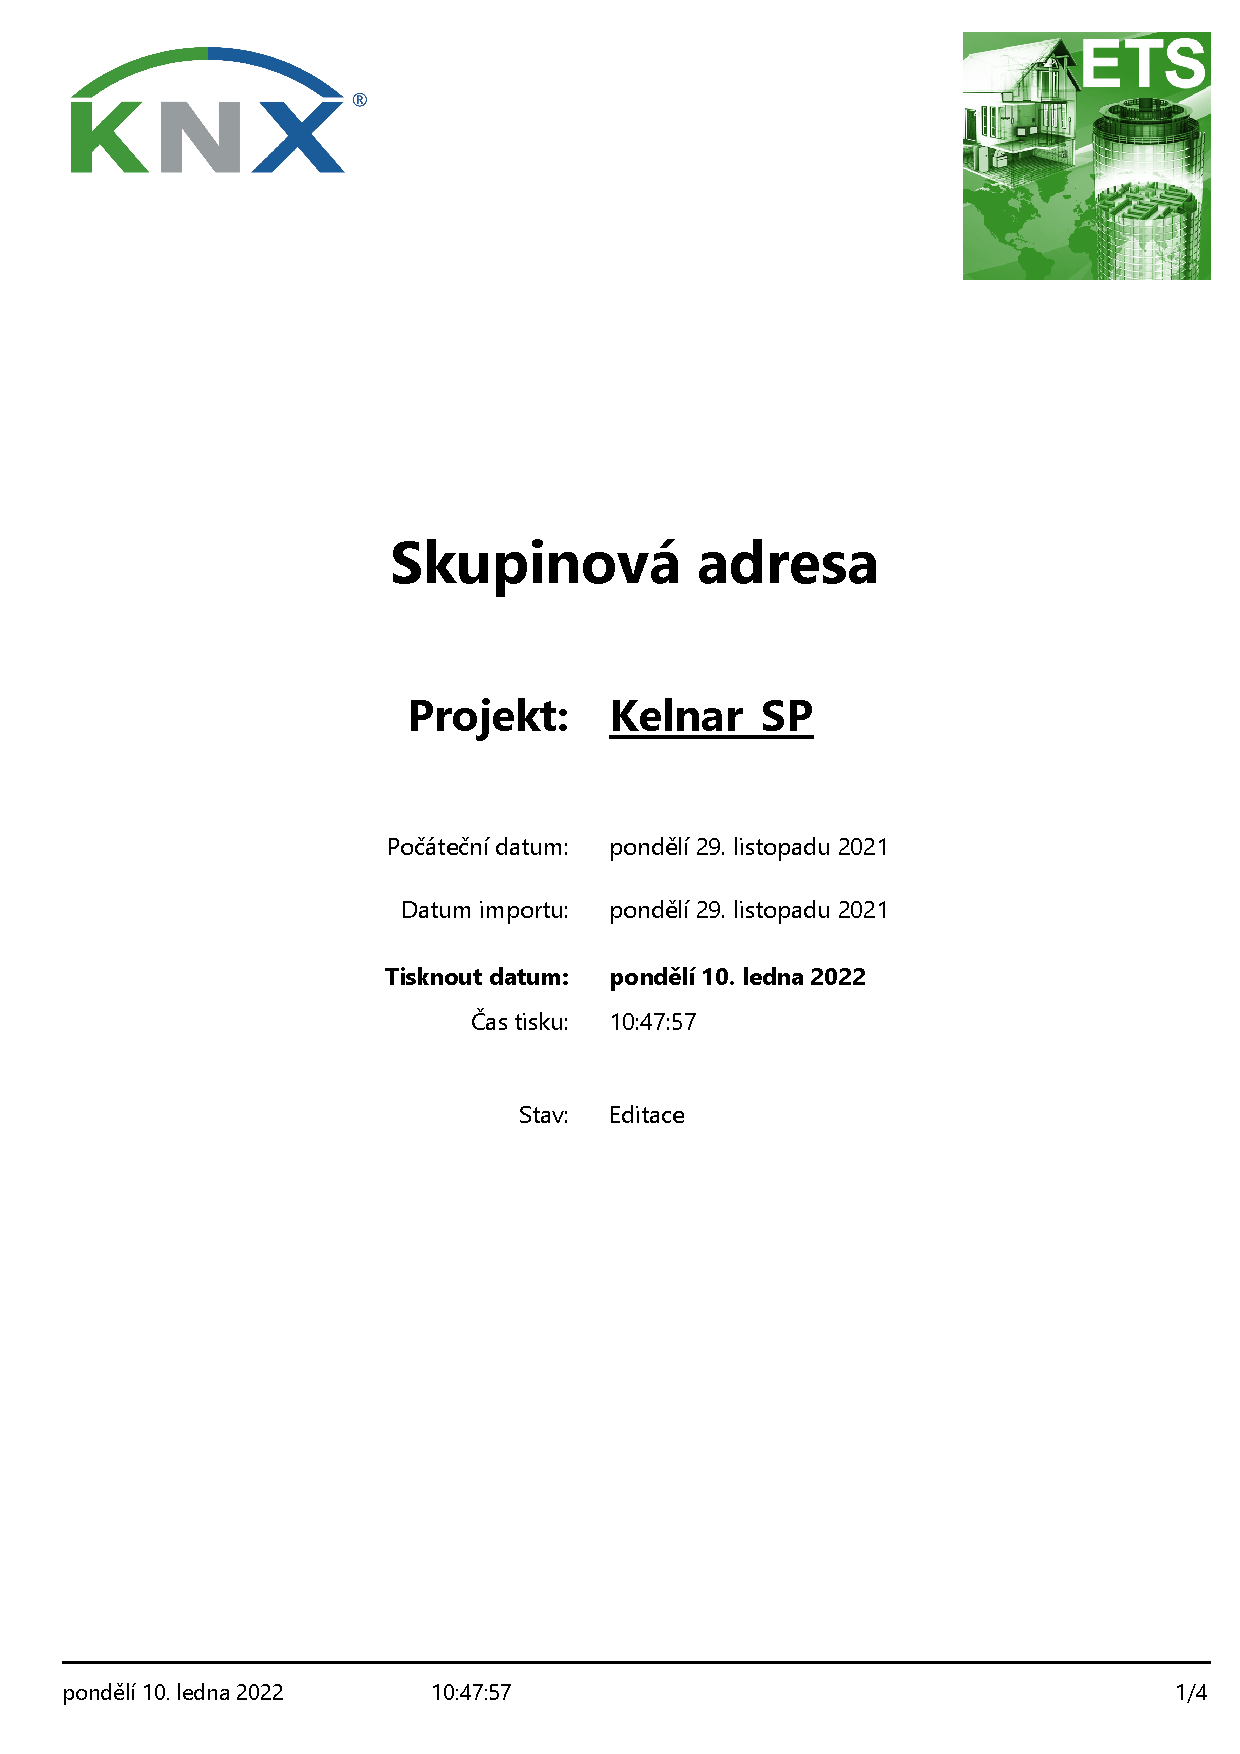
\includepdf[pages = 1]{pdf/GroupAddressesReport}
\includepdf[pages = 2]{pdf/GroupAddressesReport}
\includepdf[pages = 3]{pdf/GroupAddressesReport}
\includepdf[pages = 4]{pdf/GroupAddressesReport}
\chapter{Globální proměnné a struktury PLC}
\label{apend:globalni_promenne}
\begin{lstlisting}[language=ST, breaklines=true, numbers=left, numberstyle=\small, numbersep=10pt, frame=single, basicstyle=\ttfamily\small, caption={Globální proměnné a struktury PLC}, label={lst:globalni_promenne}]
TYPE
  DT_CMD_BOOL : STRUCT
              CMD_VAL : BOOL;
              CMD : BOOL;
  END_STRUCT;
END_TYPE
VAR_GLOBAL
  SV1_FB          : BOOL := FALSE; //KNX COMM SV1 FB
  SV2_FB          : BOOL := FALSE; //KNX COMM SV2 FB
  SV3_FB          : BOOL := FALSE; //KNX COMM SV3 FB
  SV4_FB          : BOOL := FALSE; //KNX COMM SV4 FB
  SV5_FB          : BOOL := FALSE; //KNX COMM SV5 FB
  SV6_FB          : BOOL := FALSE; //KNX COMM SV6 FB
  SV7_FB          : BOOL := FALSE; //KNX COMM SV6 FB
  SV1_CMD         : DT_CMD_BOOL; //KNX CMD SV1
  SV2_CMD         : DT_CMD_BOOL; //KNX CMD SV2
  SV3_CMD         : DT_CMD_BOOL; //KNX CMD SV3
  SV4_CMD         : DT_CMD_BOOL; //KNX CMD SV4
  SV5_CMD         : DT_CMD_BOOL; //KNX CMD SV5
  SV6_CMD         : DT_CMD_BOOL; //KNX CMD SV6
  SV7_CMD         : DT_CMD_BOOL; //KNX CMD SV6
  HEAT1_FB        : BOOL := FALSE; //KNX COMM HEAT1 FB
  HEAT2_FB        : BOOL := FALSE; //KNX COMM HEAT2 FB
  HEAT3_FB        : BOOL := FALSE; //KNX COMM HEAT3 FB
  HEAT1_CMD       : DT_CMD_BOOL; //KNX CMD HEAT1
  HEAT2_CMD       : DT_CMD_BOOL; //KNX CMD HEAT2
  HEAT3_CMD       : DT_CMD_BOOL; //KNX CMD HEAT3
  COLD1_FB        : BOOL := FALSE; //KNX COMM COLD1 FB
  COLD2_FB        : BOOL := FALSE; //KNX COMM COLD2 FB
  COLD3_FB        : BOOL := FALSE; //KNX COMM COLD3 FB
  COLD1_CMD       : DT_CMD_BOOL; //KNX CMD COLD1
  COLD2_CMD       : DT_CMD_BOOL; //KNX CMD COLD2
  COLD3_CMD       : DT_CMD_BOOL; //KNX CMD COLD3
  SHUT1_FB_UP     : BOOL := FALSE; //KNX COMM SHUT1 FB
  SHUT1_FB_DOWN   : BOOL := FALSE; //KNX COMM SHUT1 FB
  SHUT1_CMD       : DT_CMD_BOOL; //KNX CMD SHUT1
  SHUT1_STEP_CMD  : DT_CMD_BOOL; //KNX CMD SHUT1 STEP
  SHUT2_FB_UP     : BOOL := FALSE; //KNX COMM SHUT2 FB
  SHUT2_FB_DOWN   : BOOL := FALSE; //KNX COMM SHUT2 FB
  SHUT2_CMD       : DT_CMD_BOOL; //KNX CMD SHUT1
  SHUT2_STEP_CMD  : DT_CMD_BOOL; //KNX CMD SHUT1 STEP
  KNX_TEMPER      : REAL := 0.0; //KNX TEMPERATURE OUT
  OUTSIDE_TEMPER  : REAL := 0.0; //OUTSIDE TEMPER FOR MQTT
  KITCHEN_TEMPER  : REAL := 0.0; //KITCHEN TEMPER FOR MQTT
  LIVINGR_TEMPER  : REAL := 0.0; //LIVINGROOM TEMPER FOR MQTT
  BATHROOM_TEMPER : REAL := 0.0; //BATHROOM TEMPER FOR MQTT
  SHUTDOWN_MQTT   : BOOL := FALSE; //SHUTDOWN FROM MQTT
END_VAR
\end{lstlisting}
\chapter{Definice funkčního bloku fbRoomTempMod}
\label{apend:fbRoomTempMod}
\begin{lstlisting}[language=ST, breaklines=true, numbers=left, numberstyle=\small, numbersep=10pt, frame=single, basicstyle=\ttfamily\small, caption={Definice funkčního bloku fbRoomTempMod}, label={lst:fbRoomTempMod}]
FUNCTION_BLOCK fbRoomTempMod
  VAR_INPUT
    Heat_1       : BOOl; // Topení vstup 1[-]
    Heat_1_WATTS : REAL; // Topení výkon 1[W] =>[J/s]
    Heat_2       : BOOL; // Topení vstup 2[-]
    Heat_2_WATTS : REAL; // Topení výkon 2[W] =>[J/s]
    Cold_1       : BOOl; // Klimatizace vstup 1[-]
    Cold_1_WATTS : REAL; // Klimatizace výkon 1[W] =>[J/s]
    Cold_2       : BOOL; // Klimatizace vstup 2[-]
    Cold_2_WATTS : REAL; // Klimatizace výkon 2[W] =>[J/s]
    lenght       : REAL; // délka[m]
    width        : REAL; // šířka[m]
    height       : REAL; // výška[m]
    wall_temp1   : REAL; // Teplota za sousední zdí[degC]
    wall_temp2   : REAL; // Teplota za sousední zdí[degC]
    wall_temp3   : REAL; // Teplota za sousední zdí[degC]
    wall_temp4   : REAL; // Teplota za sousední zdí[degC]
    floor_temp   : REAL; // Teplota v místnosti pod[degC]
    ceiling_temp : REAL; // Teplota v místnosti nad[degC]
    wall_thic1   : REAL; // Šířka zdi1[m]
    wall_thic2   : REAL; // Šířka zdi2[m]
    wall_thic3   : REAL; // Šířka zdi3[m]
    wall_thic4   : REAL; // Šířka zdi4[m]
    floor_thic   : REAL; // Šířka podlahy[m]
    ceiling_thic : REAL; // Šířka stropu[m]
    TaskTime     : REAL; // Rychlost tasku[ms]
  END_VAR
  VAR_OUTPUT
    Temperature  : REAL := 20.0; // Teplota na výstupu[degC]
  END_VAR
  VAR
    INIT         : BOOL := FALSE; //INIT bloku
    TimeStep     : REAL := 0.0; // Hodnota kroku v ms
    VAir         : REAL := 0.0; // Obsah vzduchu[m^3]
    MAir         : REAL := 0.0; // Váha vzduchu[Kg]
    QAir         : REAL := 0.0; // Energie změna o 1degC[J]
    RoomTemp     : REAL := 20.0;// Pokojová teplota[degC]
    DeltaTemp    : REAL := 0.0; // Teplota za cyklus[degC]
    KHeatRise    : REAL := 2.4; // Korekční člen tr[-]
    KColdRise    : REAL := 45.0;// Korekční člen kr[-]
    KHeatFall1   : REAL := 0.0; // Korekční člen tf 1[-]
    KColdFall1   : REAL := 0.0; // Korekční člen kf 1[-]
    KHeatFall2   : REAL := 0.0; // Korekční člen tf 2[-]
    KColdFall2   : REAL := 0.0; // Korekční člen kf 2[-]
    Epsilon      : REAL := 1.0; // Sp výkon za čas[w]
    AlphaHeat    : REAL := 0.0; // Logaritmus topení[-]
    AlphaCold    : REAL := 0.0; // Logaritmus klimatizace[-]
    FiTotal      : REAL := 0.0; // Celkový tepelný tok[J/s]
    FiHeat       : REAL := 0.0; // Celkový tepelný tok t[J/s]
    FiHeatTmp1   : REAL := 0.0; // Tepelný tok topení 1[J/s]
    FiHeatTmp2   : REAL := 0.0; // Tepelný tok topení 2[J/s]
    FiCold       : REAL := 0.0; // Celkový tepelný tok k[J/s]
    FiColdTmp1   : REAL := 0.0; // Tepelný tok klim 1[J/s]
    FiColdTmp2   : REAL := 0.0; // Tepelný tok klim 2[J/s]
    AreaWall1    : REAL := 0.0; // Plocha zdi 1[m^2]
    AreaWall2    : REAL := 0.0; // Plocha zdi 2[m^2]
    AreaWall3    : REAL := 0.0; // Plocha zdi 3[m^2]
    AreaWall4    : REAL := 0.0; // Plocha zdi 4[m^2]
    AreaFloor    : REAL := 0.0; // Plocha podlahy[m^2]
    AreaCeiling  : REAL := 0.0; // Plocha stropu[m^2]
  END_VAR
  VAR_TEMP
    DeltaTempWall_1     : REAL := 0; // Rozdíl 1[degC]
    DeltaTempWall_2     : REAL := 0; // Rozdíl 2[degC]
    DeltaTempWall_3     : REAL := 0; // Rozdíl 3[degC]
    DeltaTempWall_4     : REAL := 0; // Rozdíl 4[degC]
    DeltaTempFloor      : REAL := 0; // Rozdíl podlaha[degC]
    DeltaTempCeiling    : REAL := 0; // Rozdíl strop[degC]
    FiWall_1     : REAL := 0.0; // Tepelný tok 1[J/s]
    FiWall_2     : REAL := 0.0; // Tepelný tok 2[J/s]
    FiWall_3     : REAL := 0.0; // Tepelný tok 3[J/s]
    FiWall_4     : REAL := 0.0; // Tepelný tok 4[J/s]
    FiFloor      : REAL := 0.0; // Tepelný tok podlaha[J/s]
    FiCeiling    : REAL := 0.0; // Tepelný tok strop[J/s]
  END_VAR
  VAR CONSTANT
    RoAir : REAL := 1.204; // Hustota vzduchu[Kg/m^3]
    CpAir : REAL := 1005.0; // Tepelná kap vzduchu[J/(kg*K)]
    LambdaBrick  : REAL := 0.4; // Tepelná vod cihly[W/(m*K)]
    MaxTemp      : REAL := 24.0; // Maximální teplota[degC]
    MinTemp      : REAL := 16.0; // Minimální teplota[degC]
    TimeRise     : REAL := 15.0; // Čas náběhu výkonu[s]
    TimeFallHeat : REAL := 15.0; // Čas klesání výkonu t[s]
    TimeFallCold : REAL := 10.0; // Čas klesání výkonu k[s]
    TargTimeHeat : REAL := 5.06; // Čas na dosažení 80% t[s]
    TargTimeCold : REAL := 3.29; // Čas na dosažení 80% k[s]
  END_VAR
IF NOT(INIT) THEN
   TimeStep := TaskTime / 1000.0; // ms => s
END_IF;

(* Výpočet objemu, hmotnosti, energie *)
IF NOT(INIT) THEN
  VAir := lenght * width * height;
  MAir := RoAir * VAir;
  QAir := MAir * CpAir;
END_IF;

(* Výpočet ploch *)
IF NOT(INIT) THEN
  AreaWall1 := height * width;
  AreaWall2 := height * width;
  AreaWall3 := height * lenght;
  AreaWall4 := height * lenght;
  AreaFloor := lenght * width;
  AreaCeiling := lenght 
  
(* Výpočet deltaT *)
DeltaTempWall_1 := wall_temp1 - RoomTemp;
DeltaTempWall_2 := wall_temp2 - RoomTemp;
DeltaTempWall_3 := wall_temp3 - RoomTemp;
DeltaTempWall_4 := wall_temp4 - RoomTemp;
DeltaTempFloor := floor_temp - RoomTemp;
DeltaTempCeiling := ceiling_temp - RoomTemp;

(* Výpočet tepelných toků přes stěny *)
FiWall_1 := (LambdaBrick * AreaWall1 * DeltaTempWall_1) / wall_thic1;
FiWall_2 := (LambdaBrick * AreaWall2 * DeltaTempWall_2) / wall_thic2;
FiWall_3 := (LambdaBrick * AreaWall3 * DeltaTempWall_3) / wall_thic3;
FiWall_4 := (LambdaBrick * AreaWall4 * DeltaTempWall_4) / wall_thic4;
FiFloor := (LambdaBrick * AreaFloor * DeltaTempFloor) / floor_thic;
FiCeiling := (LambdaBrick * AreaCeiling * DeltaTempCeiling)/ceiling_thic;

(* Výpočet korekčních členu *)
IF NOT(INIT) THEN
  KHeatRise := (TimeRise / TargTimeHeat) - 1.0;
  KColdRise := (TimeRise / TargTimeCold) - 1.0;
  KHeatFall1 := (LN(Heat_1_WATTS/Epsilon))/TimeFallHeat;
  KHeatFall2 := (LN(Heat_2_WATTS/Epsilon))/TimeFallHeat;
  KColdFall1 := (LN(Cold_1_WATTS/Epsilon))/TimeFallCold;
  KColdFall2 := (LN(Cold_2_WATTS/Epsilon))/TimeFallCold;
END_IF;

(* Tepelný výkon topení a klimatizace *)
(* Výpočet alfy *)
IF NOT(INIT) THEN
  AlphaHeat := LN(1 + KHeatRise * (TimeStep)) / LN(1 + KHeatRise * TimeRise);
  AlphaCold := LN(1 + KColdRise * (TimeStep)) / LN(1 + KColdRise * TimeRise);
END_IF;

(* Topení 1 *)
IF Heat_1 THEN
  FiHeatTmp1 := FiHeatTmp1 + AlphaHeat * (Heat_1_WATTS - FiHeatTmp1);
ELSE
  FiHeatTmp1 := FiHeatTmp1 * EXP(-KHeatFall1 * (TimeStep));
END_IF;
(* Topení 2 *)
IF Heat_2 THEN
  FiHeatTmp2 := FiHeatTmp2 + AlphaHeat * (Heat_2_WATTS - FiHeatTmp2);
ELSE
  FiHeatTmp2 := FiHeatTmp2 * EXP(-KHeatFall2 * (TimeStep));
END_IF;
(* Klimatizace 1 *)
IF Cold_1 THEN
  FiColdTmp1 := FiColdTmp1 + AlphaCold * (Cold_1_WATTS - FiColdTmp1);
ELSE
  FiColdTmp1 := FiColdTmp1 * EXP(-KColdFall1 * (TimeStep));
END_IF;
(* Klimatizace 2 *)
IF Cold_2 THEN
  FiColdTmp2 := FiColdTmp2 + AlphaCold * (Cold_2_WATTS - FiColdTmp2);
ELSE
  FiColdTmp2 := FiColdTmp2 * EXP(-KColdFall2 * (TimeStep));
END_IF;

(* Suma výkonů *)
FiHeat := FiHeatTmp1 + FiHeatTmp2;
FiCold := FiColdTmp1 + FiColdTmp2;

(* Celkový tepelný tok *)
FiTotal := FiHeat - FiCold + FiWall_1 + FiWall_2 + FiWall_3 + FiWall_4 + FiFloor + FiCeiling;

(* Výpočet přírůstku teploty za task *)
DeltaTemp := (FiTotal / QAir) * TimeStep;
RoomTemp := RoomTemp + DeltaTemp;

(* Výstup *)
Temperature := RoomTemp;

(* NOT INIT *)
INIT := TRUE;
END_FUNCTION_BLOCK
\end{lstlisting}
\newpage
\chapter{Popis funkčního bloku fbBath}
\label{apend:fbBath}
\begin{lstlisting}[language=ST, breaklines=true, numbers=left, numberstyle=\small, numbersep=10pt, frame=single, basicstyle=\ttfamily\small, caption={Definice funkčního bloku fbBath}, label={lst:fbBath}]
  FUNCTION_BLOCK fbBath
  VAR_INPUT
    SV6_ON       : BOOl; //Vizu světlo 6 on
    SV6_OFF      : BOOl; //Vizu světlo 6 off
    SV6_KNX_FB   : BOOl; //KNX světlo 6 feedback
  END_VAR
  VAR_OUTPUT
    SV6          : BOOL;   //Vizualizace světla 6
    SV6_CMD      : DT_CMD_BOOL;   //Příkaz světla 6
    TemperBath   : REAL;   //Vizualizace + komunikace
  END_VAR
  VAR
    Time_s   : REAL := 0.0;
    fbSV6 : fbKNXVisuBool;
  END_VAR
  VAR CONSTANT
    PI       : REAL := 3.14159265;
    Freq     : REAL := 0.005; // perioda cca 3 minuty 20 sekund
    TaskTime : REAL := 400.0; // 250 ms
  END_VAR
\end{lstlisting}
\begin{figure}[!ht]
  \begin{center}
  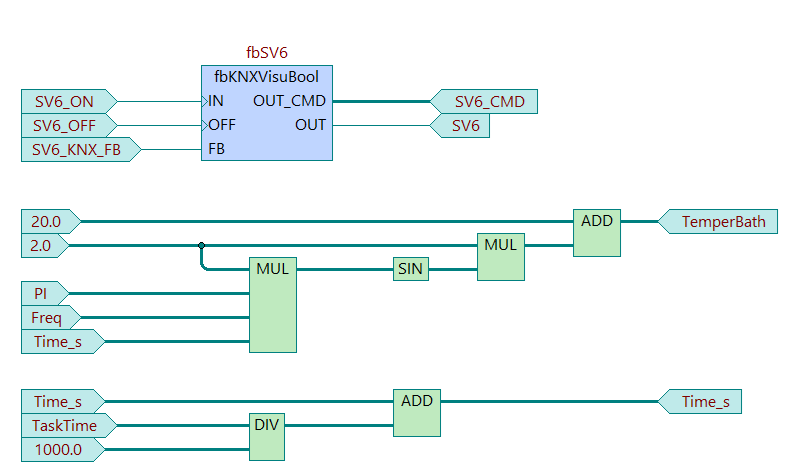
\includegraphics[scale=0.55]{obrazky/fbBath.png}
  \end{center}
  \caption[Logika funkčního bloku fbBath]{Logika funkčního bloku fbBath}
  \label{fig:fbBath}
\end{figure}
\pagebreak
\newpage
\chapter{Definice funkčního bloku fbKitch}
\label{apend:fbKitch}
\begin{lstlisting}[language=ST, breaklines=true, numbers=left, numberstyle=\small, numbersep=10pt, frame=single, basicstyle=\ttfamily\small, caption={Definice funkčního bloku fbKitch}, label={lst:fbKitch}]
  FUNCTION_BLOCK fbKitch
  VAR_INPUT
    SV1_ON         : BOOl; //Vizu světlo 1 on
    SV1_OFF        : BOOl; //Vizu světlo 1 off
    SV1_KNX_FB     : BOOl; //KNX světlo 1 feedback,
    SV2_ON         : BOOl; //Vizu světlo 2 on
    SV2_OFF        : BOOl; //Vizu světlo 2 off
    SV2_KNX_FB     : BOOl; //KNX světlo 2 feedback
    Heater3_ON     : BOOl; //Vizu topení 3 on
    Heater3_OFF    : BOOl; //Vizu topení 3 off
    Heater3_KNX_FB : BOOl; //KNX klimatizace 3 feedback
    Climat3_ON     : BOOl; //Vizu klimatizace 3 on
    Climat3_OFF    : BOOl; //Vizu klimatizace 3 off
    Climat3_KNX_FB : BOOl; //KNX topení 3 feedback
    wall_temp1     : REAL; // Teplota koupelna[degC]
    wall_temp2     : REAL; // Teplota ven[degC]
    wall_temp3     : REAL; // Teplota ven[degC]
    wall_temp4     : REAL; // Teplota ven[degC]
    ceiling_temp   : REAL; // Teplota obyvak[degC]
  END_VAR
  VAR_OUTPUT
    SV1            : BOOL;   //Vizualizace světla 1
    SV2            : BOOL;   //Vizualizace světla 2
    Heater3        : BOOL;   //Vizualizace topení 3
    Climat3        : BOOL;   //Vizualizace klimatizace 3
    SV1_CMD        : DT_CMD_BOOL;   //Příkaz světla 1
    SV2_CMD        : DT_CMD_BOOL;   //Příkaz světla 2
    Heater3_CMD    : DT_CMD_BOOL;   //Příkaz topení 3
    Climat3_CMD    : DT_CMD_BOOL;   //Příkaz klimatizace 3
    TemperKitchen  : REAL;   //Vizualizace + komunikace
  END_VAR
  VAR
    fbSV1 : fbKNXVisuBool;
    fbSV2 : fbKNXVisuBool;
    fbHeater3 : fbKNXVisuBool;
    fbKitchMod : fbRoomTempMod;
    fbClimat3 : fbKNXVisuBool;
  END_VAR
\end{lstlisting}
\begin{figure}[!ht]
  \begin{center}
  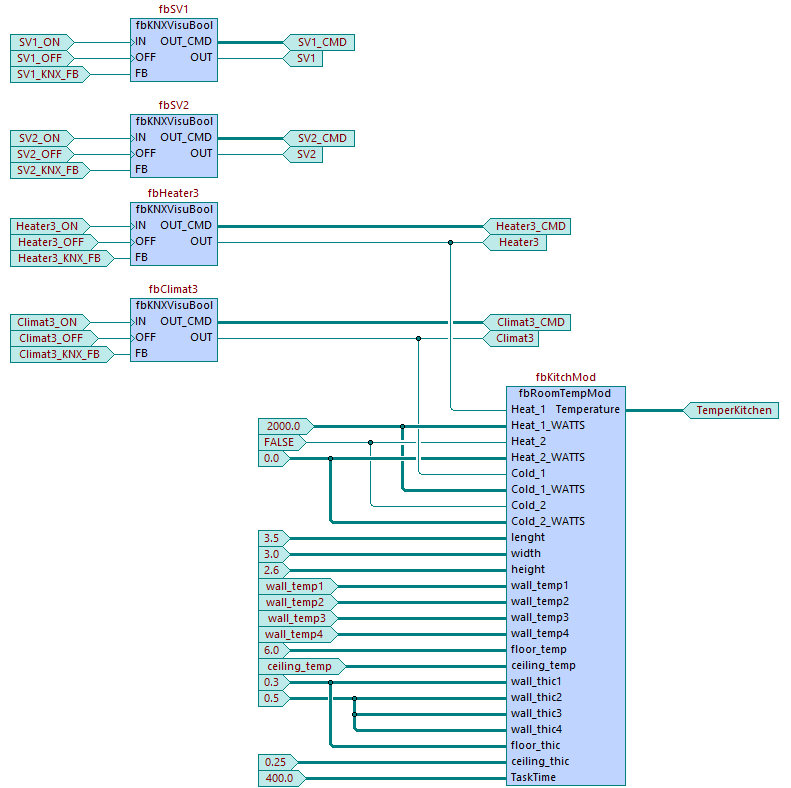
\includegraphics[scale=0.7]{obrazky/fbKitch.png}
  \end{center}
  \caption[Logika funkčního bloku fbKitch]{Logika funkčního bloku fbKitch}
  \label{fig:fbKitch}
\end{figure}
\pagebreak
\chapter{Definice funkčního bloku fbLivRoom}
\label{apend:fbLivRoom}
\begin{lstlisting}[language=ST, breaklines=true, numbers=left, numberstyle=\small, numbersep=10pt, frame=single, basicstyle=\ttfamily\small, caption={Definice funkčního bloku fbLivRoom}, label={lst:fbLivRoom}]
FUNCTION_BLOCK fbLivRoom
  VAR_INPUT
    SV3_ON          : BOOl; //Vizu světlo 3 on
    SV3_OFF         : BOOl; //Vizu světlo 3 off
    SV3_KNX_FB      : BOOl; //KNX světlo 3 feedback,
    SV4_ON          : BOOl; //Vizu světlo 4 on
    SV4_OFF         : BOOl; //Vizu světlo 4 off
    SV4_KNX_FB      : BOOl; //KNX světlo 4 feedback
    SV5_ON          : BOOl; //Vizu světlo 5 on
    SV5_OFF         : BOOl; //Vizu světlo 5 off
    SV5_KNX_FB      : BOOl; //KNX světlo 5 feedback
    Shut1_UP        : BOOl; //Vizu rolety 1 on
    Shut1_DW        : BOOl; //Vizu rolety 1 down
    Shut1_STEP_UP   : BOOl; //Vizu rolety 1 on krok
    Shut1_STEP_DW   : BOOl; //Vizu rolety 1 off krok
    Shut1_KNX_FB_UP : BOOl; //KNX rolety 1 feedback up
    Shut1_KNX_FB_DW : BOOl; //KNX rolety 1 feedback down
    Shut2_UP        : BOOl; //Vizu rolety 2 on
    Shut2_DW        : BOOl; //Vizu rolety 2 down
    Shut2_STEP_UP   : BOOl; //Vizu rolety 2 on krok
    Shut2_STEP_DW   : BOOl; //Vizu rolety 2 off krok
    Shut2_KNX_FB_UP : BOOl; //KNX rolety 2 feedback up
    Shut2_KNX_FB_DW : BOOl; //KNX rolety 2 feedback down
    Heater1_ON      : BOOl; //Vizu topení 1 on
    Heater1_OFF     : BOOl; //Vizu topení 1 off
    Heater1_KNX_FB  : BOOl; //KNX klimatizace 1 feedback
    Heater2_ON      : BOOl; //Vizu topení 2 on
    Heater2_OFF     : BOOl; //Vizu topení 2 off
    Heater2_KNX_FB  : BOOl; //KNX klimatizace 2 feedback
    Climat1_ON      : BOOl; //Vizu klimatizace 1 on
    Climat1_OFF     : BOOl; //Vizu klimatizace 1 off
    Climat1_KNX_FB  : BOOl; //KNX topení 1 feedback
    Climat2_ON      : BOOl; //Vizu klimatizace 2 on
    Climat2_OFF     : BOOl; //Vizu klimatizace 2 off
    Climat2_KNX_FB  : BOOl; //KNX topení 2 feedback
    wall_temp1      : REAL; // Teplota koupelna[degC]
    wall_temp2      : REAL; // Teplota ven[degC]
    wall_temp3      : REAL; // Teplota ven[degC]
    wall_temp4      : REAL; // Teplota ven[degC]
    floor_temp      : REAL; // Teplota v místnosti pod[degC]
    ceiling_temp    : REAL; // Teplota obyvak[degC]
  END_VAR
  VAR_OUTPUT
    SV3          : BOOL;   //Vizualizace světla 3
    SV4          : BOOL;   //Vizualizace světla 4
    SV5          : BOOL;   //Vizualizace světla 5
    SV3_CMD      : DT_CMD_BOOL;   //Příkaz světla 3
    SV4_CMD      : DT_CMD_BOOL;   //Příkaz světla 4
    SV5_CMD      : DT_CMD_BOOL;   //Příkaz světla 5
    Heater1        : BOOL;   //Vizualizace topení 1
    Heater2        : BOOL;   //Vizualizace topení 2
    Heater1_CMD    : DT_CMD_BOOL;   //Příkaz topení 1
    Heater2_CMD    : DT_CMD_BOOL;   //Příkaz topení 2
    Climat1        : BOOL;   //Vizualizace klimatizace 1
    Climat2        : BOOL;   //Vizualizace klimatizace 2
    Climat1_CMD    : DT_CMD_BOOL;   //Příkaz klimatizace 1
    Climat2_CMD    : DT_CMD_BOOL;   //Příkaz klimatizace 2
    Shut1_UP_OUT   : BOOL;   //Vizualizace žaluzie 1 UP
    Shut1_DOWN_OUT : BOOL;   //Vizualizace žaluzie 1 DOWN
    Shut1_CMD      : DT_CMD_BOOL;   //Příkaz žaluzie 1
    Shut1_STEP_CMD : DT_CMD_BOOL;   //Příkaz žaluzie 1 KROK
    Shut2_UP_OUT   : BOOL;   //Vizualizace žaluzie 2 UP
    Shut2_DOWN_OUT : BOOL;   //Vizualizace žaluzie 2 DOWN
    Shut2_CMD      : DT_CMD_BOOL;   //Příkaz žaluzie 2
    Shut2_STEP_CMD : DT_CMD_BOOL;   //Příkaz žaluzie 2 KROK
    TemperLivingR  : REAL;   //Vizualizace + komunikace
  END_VAR
  VAR
    fbSV3 : fbKNXVisuBool;
    fbSV4 : fbKNXVisuBool;
    fbSV5 : fbKNXVisuBool;
    fbHeater1 : fbKNXVisuBool;
    fbClimat1 : fbKNXVisuBool;
    fbHeater2 : fbKNXVisuBool;
    fbClimat2 : fbKNXVisuBool;
    fbLivingRMod : fbRoomTempMod;
    fbShut1 : fbKNXShutters;
    fbShut2 : fbKNXShutters;
  END_VAR
\end{lstlisting}
\begin{figure}[!ht]
  \begin{center}
  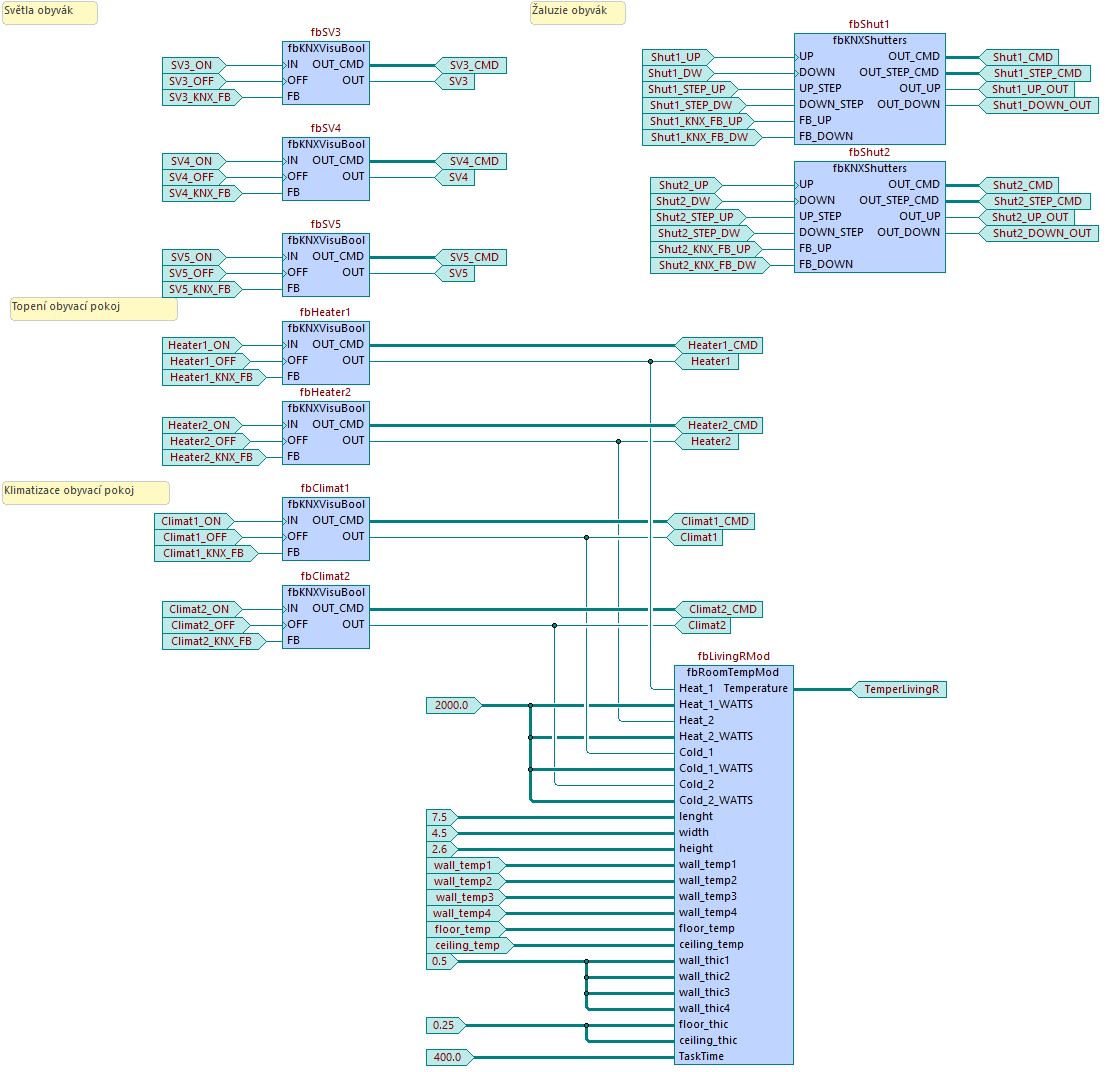
\includegraphics[scale=0.6]{obrazky/fbLivRoom.png}
  \end{center}
  \caption[Logika funkčního bloku fbLivRoom]{Logika funkčního bloku fbLivRoom}
  \label{fig:fbLivRoom}
\end{figure}
\pagebreak
\chapter{Definice funkčního bloku fbOutz}
\label{apend:fbOutz}
\begin{lstlisting}[language=ST, breaklines=true, numbers=left, numberstyle=\small, numbersep=10pt, frame=single, basicstyle=\ttfamily\small, caption={Definice funkčního bloku fbOutz}, label={lst:fbOutz}]
  FUNCTION_BLOCK fbOutz
  VAR_INPUT
    SV7_ON       : BOOl R_EDGE; //Vizu světlo 7 on
    SV7_OFF      : BOOl R_EDGE; //Vizu světlo 7 off
    SV7_KNX_FB   : BOOl; //KNX světlo 7 feedback
    KNX_OUT_TEMP : REAL; // KNX Teplota venku
  END_VAR
  VAR_OUTPUT
    SV7          : BOOL;   //Vizualizace světla 7
    SV7_CMD      : DT_CMD_BOOL;   //Příkaz světla 7
    TemperOut    : REAL;   //Vizualizace + komunikace
  END_VAR
  VAR_IN_OUT
  END_VAR
  VAR
    fbSV7 : fbKNXVisuBool;
  END_VAR
  VAR_TEMP
  END_VAR
\end{lstlisting}
\begin{figure}[!ht]
  \begin{center}
  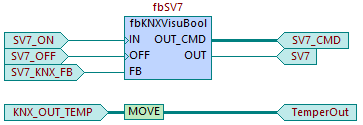
\includegraphics[scale=1.0]{obrazky/fbOutz.png}
  \end{center}
  \caption[Logika funkčního bloku fbOutz]{Logika funkčního bloku fbOutz}
  \label{fig:fbOutz}
\end{figure}
\pagebreak
\chapter{Program komunikace mezi PLC a KNX}
\label{apend:KNXComm}
\begin{lstlisting}[language=ST, breaklines=true, numbers=left, numberstyle=\small, numbersep=10pt, frame=single, basicstyle=\ttfamily\small, caption={Program komunikace mezi PLC a KNX}, label={lst:prgKNXComm}]
  PROGRAM prgKNXComm
  VAR
    init : BOOL;
    knx  : fbKnxIpBaosBin;
    knxObjectList    : ARRAY[1..34] OF UDINT; // pole adres
    SHUT1_FB_PULSE : TON;
    SHUT2_FB_PULSE : TON;
    datapoint1       : T_KNX_OBJECT_DPT1;  // SV1_FB
    datapoint2       : T_KNX_OBJECT_DPT1;  // SV2_FB
    datapoint3       : T_KNX_OBJECT_DPT1;  // SV3_FB
    datapoint4       : T_KNX_OBJECT_DPT1;  // SV4_FB
    datapoint5       : T_KNX_OBJECT_DPT1;  // SV5_FB
    datapoint6       : T_KNX_OBJECT_DPT1;  // SV6_FB
    datapoint7       : T_KNX_OBJECT_DPT1;  // SV7_FB
    datapoint8       : T_KNX_OBJECT_DPT1;  // HEAT1_FB
    datapoint9       : T_KNX_OBJECT_DPT1;  // HEAT2_FB
    datapoint10      : T_KNX_OBJECT_DPT1;  // HEAT3_FB
    datapoint11      : T_KNX_OBJECT_DPT1;  // COLD1_FB
    datapoint12      : T_KNX_OBJECT_DPT1;  // COLD2_FB
    datapoint13      : T_KNX_OBJECT_DPT1;  // COLD3_FB
    datapoint14      : T_KNX_OBJECT_DPT1;  // SHUT1_FB
    datapoint15      : T_KNX_OBJECT_DPT1;  // SHUT1_CMD
    datapoint16      : T_KNX_OBJECT_DPT1;  // SHUT2_FB
    datapoint17      : T_KNX_OBJECT_DPT1;  // SHUT2_CMD
    datapoint18      : T_KNX_OBJECT_DPT1;  // SV1_CMD
    datapoint19      : T_KNX_OBJECT_DPT1;  // SV2_CMD
    datapoint20      : T_KNX_OBJECT_DPT1;  // SV3_CMD
    datapoint21      : T_KNX_OBJECT_DPT1;  // SV4_CMD
    datapoint22      : T_KNX_OBJECT_DPT1;  // SV5_CMD
    datapoint23      : T_KNX_OBJECT_DPT1;  // SV6_CMD
    datapoint24      : T_KNX_OBJECT_DPT1;  // SV7_CMD
    datapoint25      : T_KNX_OBJECT_DPT1;  // HEAT1_CMD
    datapoint26      : T_KNX_OBJECT_DPT1;  // HEAT2_CMD
    datapoint27      : T_KNX_OBJECT_DPT1;  // HEAT3_CMD
    datapoint28      : T_KNX_OBJECT_DPT1;  // COLD1_CMD
    datapoint29      : T_KNX_OBJECT_DPT1;  // COLD2_CMD
    datapoint30      : T_KNX_OBJECT_DPT1;  // COLD3_CMD
    datapoint31      : T_KNX_OBJECT_DPT1;  // krok Ž 1
    datapoint32      : T_KNX_OBJECT_DPT1;  // krok Ž 2
    datapoint33      : T_KNX_OBJECT_DPT18; // scéna
    datapoint34      : T_KNX_OBJECT_DPT9;  // teplota
  END_VAR
IF NOT init THEN // pole adres
  knxObjectList[1]  := PTR_TO_UDINT( ADR(datapoint1));   
  knxObjectList[2]  := PTR_TO_UDINT( ADR(datapoint2));   
  knxObjectList[3]  := PTR_TO_UDINT( ADR(datapoint3));   
  knxObjectList[4]  := PTR_TO_UDINT( ADR(datapoint4));   
  knxObjectList[5]  := PTR_TO_UDINT( ADR(datapoint5));   
  knxObjectList[6]  := PTR_TO_UDINT( ADR(datapoint6));   
  knxObjectList[7]  := PTR_TO_UDINT( ADR(datapoint7));   
  knxObjectList[8]  := PTR_TO_UDINT( ADR(datapoint8));   
  knxObjectList[9]  := PTR_TO_UDINT( ADR(datapoint9));   
  knxObjectList[10] := PTR_TO_UDINT( ADR(datapoint10));  
  knxObjectList[11] := PTR_TO_UDINT( ADR(datapoint11));  
  knxObjectList[12] := PTR_TO_UDINT( ADR(datapoint12));  
  knxObjectList[13] := PTR_TO_UDINT( ADR(datapoint13));  
  knxObjectList[14] := PTR_TO_UDINT( ADR(datapoint14));  
  knxObjectList[15] := PTR_TO_UDINT( ADR(datapoint15));  
  knxObjectList[16] := PTR_TO_UDINT( ADR(datapoint16));  
  knxObjectList[17] := PTR_TO_UDINT( ADR(datapoint17));  
  knxObjectList[18] := PTR_TO_UDINT( ADR(datapoint18));  
  knxObjectList[19] := PTR_TO_UDINT( ADR(datapoint19));  
  knxObjectList[20] := PTR_TO_UDINT( ADR(datapoint20));  
  knxObjectList[21] := PTR_TO_UDINT( ADR(datapoint21));  
  knxObjectList[22] := PTR_TO_UDINT( ADR(datapoint22));  
  knxObjectList[23] := PTR_TO_UDINT( ADR(datapoint23));  
  knxObjectList[24] := PTR_TO_UDINT( ADR(datapoint24));  
  knxObjectList[25] := PTR_TO_UDINT( ADR(datapoint25));  
  knxObjectList[26] := PTR_TO_UDINT( ADR(datapoint26));  
  knxObjectList[27] := PTR_TO_UDINT( ADR(datapoint27));  
  knxObjectList[28] := PTR_TO_UDINT( ADR(datapoint28));  
  knxObjectList[29] := PTR_TO_UDINT( ADR(datapoint29));  
  knxObjectList[30] := PTR_TO_UDINT( ADR(datapoint30));    
  knxObjectList[31] := PTR_TO_UDINT( ADR(datapoint31));
  knxObjectList[32] := PTR_TO_UDINT( ADR(datapoint32));  
  knxObjectList[33] := PTR_TO_UDINT( ADR(datapoint33));    
  knxObjectList[34] := PTR_TO_UDINT( ADR(datapoint34));   
  init := TRUE;
END_IF
knx( firstKnxObject := 1,
     lastKnxObject := 34,
     ethCode := ETH2_uni2,
     knxIP := STRING_TO_IPADR('192.168.xxx.xx'),
     knxList := void( knxObjectList));

// Feedbacky
SV1_FB       := datapoint1 .value;
SV2_FB       := datapoint2 .value;
SV3_FB       := datapoint3 .value;
SV4_FB       := datapoint4 .value;
SV5_FB       := datapoint5 .value;
SV6_FB       := datapoint6 .value;
SV7_FB       := datapoint7 .value;
HEAT1_FB     := datapoint8 .value;
HEAT2_FB     := datapoint9 .value;
HEAT3_FB     := datapoint10.value;
COLD1_FB     := datapoint11.value;
COLD2_FB     := datapoint12.value;
COLD3_FB     := datapoint13.value;
SHUT1_FB_PULSE(IN := datapoint14.altValue, PT := T#1s);
SHUT2_FB_PULSE(IN := datapoint16.altValue, PT := T#1s);
SHUT1_FB_UP   := datapoint14.value AND SHUT1_FB_PULSE.Q;
SHUT1_FB_DOWN := NOT(datapoint14.value) AND SHUT1_FB_PULSE.Q;
SHUT2_FB_UP   := datapoint16.value AND SHUT2_FB_PULSE.Q;
SHUT2_FB_DOWN := NOT(datapoint16.value) AND SHUT2_FB_PULSE.Q;

// Příkazy
IF SV1_CMD.CMD       THEN datapoint18.value := SV1_CMD.CMD_VAL; END_IF;
IF SV2_CMD.CMD       THEN datapoint19.value := SV2_CMD.CMD_VAL; END_IF;
IF SV3_CMD.CMD       THEN datapoint20.value := SV3_CMD.CMD_VAL; END_IF;
IF SV4_CMD.CMD       THEN datapoint21.value := SV4_CMD.CMD_VAL; END_IF;
IF SV5_CMD.CMD       THEN datapoint22.value := SV5_CMD.CMD_VAL; END_IF;
IF SV6_CMD.CMD       THEN datapoint23.value := SV6_CMD.CMD_VAL; END_IF;
IF SV7_CMD.CMD       THEN datapoint24.value := SV7_CMD.CMD_VAL; END_IF;
IF HEAT1_CMD.CMD     THEN datapoint25.value := HEAT1_CMD.CMD_VAL; END_IF;
IF HEAT2_CMD.CMD     THEN datapoint26.value := HEAT2_CMD.CMD_VAL; END_IF;
IF HEAT3_CMD.CMD     THEN datapoint27.value := HEAT3_CMD.CMD_VAL; END_IF;
IF COLD1_CMD.CMD     THEN datapoint28.value := COLD1_CMD.CMD_VAL; END_IF;
IF COLD2_CMD.CMD     THEN datapoint29.value := COLD2_CMD.CMD_VAL; END_IF;
IF COLD3_CMD.CMD     THEN datapoint30.value := COLD3_CMD.CMD_VAL; END_IF;
IF SHUT1_CMD.CMD     THEN datapoint15.value  := SHUT1_CMD.CMD_VAL; END_IF;
IF SHUT1_STEP_CMD.CMD THEN datapoint31.value := SHUT1_STEP_CMD.CMD_VAL; END_IF;
IF SHUT2_CMD.CMD     THEN datapoint17.value  := SHUT1_CMD.CMD_VAL; END_IF;
IF SHUT2_STEP_CMD.CMD THEN datapoint32.value := SHUT1_STEP_CMD.CMD_VAL; END_IF;
// Shutdown scéna
IF SHUTDOWN_MQTT THEN
  datapoint33.control := TRUE;
  datapoint33.scene   := 5;
END_IF
// Posílání teploty
KNX_TEMPER := datapoint34.value;
END_PROGRAM
\end{lstlisting}
\chapter{Program komunikace mezi PLC a Home Assistant - MQTT}
\label{apend:MQTTComm}
\begin{lstlisting}[language=ST, breaklines=true, numbers=left, numberstyle=\small, numbersep=10pt, frame=single, basicstyle=\ttfamily\small, caption={Program komunikace mezi PLC a Home Assistant - MQTT}, label={lst:prgMQTTComm}]

\end{lstlisting}
\chapter{Vizualizace PLC}
\label{apend:vizualizace}
\begin{figure}[!ht]
  \begin{center}
  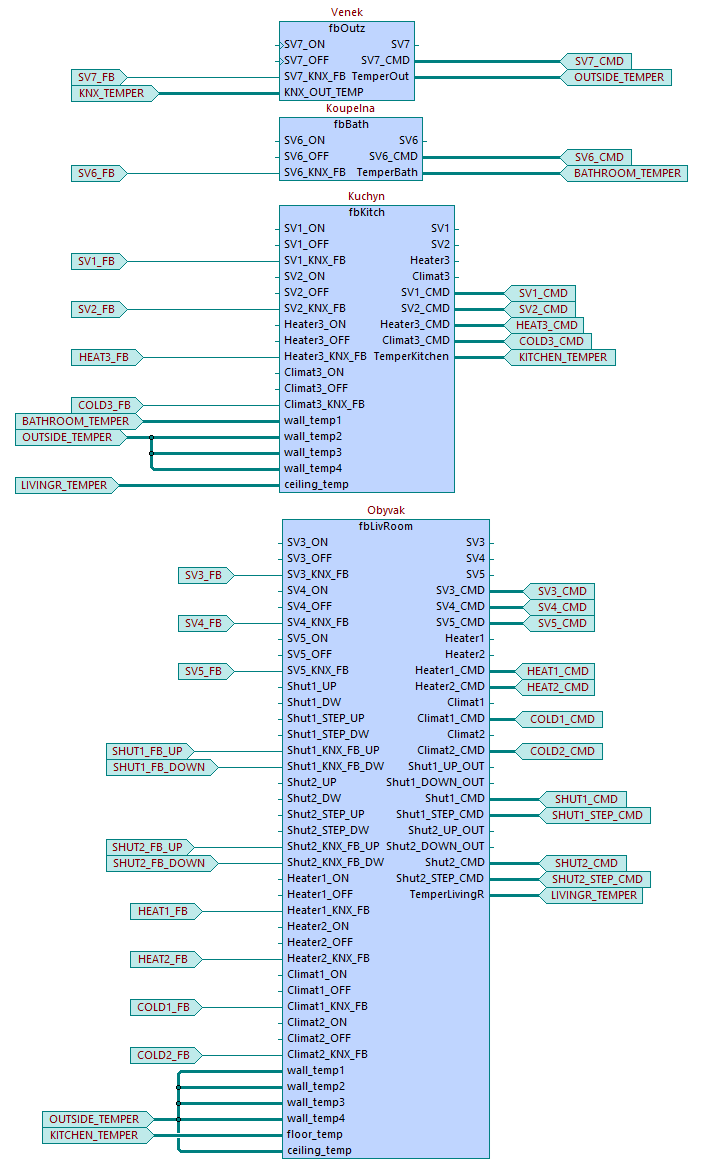
\includegraphics[scale=0.65]{obrazky/prgVizu.png}
  \end{center}
  \caption[Vizualizace PLC]{Vizualizace PLC}
  \label{fig:vizualizace}
\end{figure}
\begin{figure}[!ht]
  \begin{center}
  \includegraphics[scale=0.8]{obrazky/Přehled.png}
  \end{center}
  \caption[WebMaker - Hlavní obrazovka]{WebMaker - Hlavní obrazovka}
  \label{fig:hlavniObrazovka}
\end{figure}
\begin{figure}[!ht]
  \begin{center}
  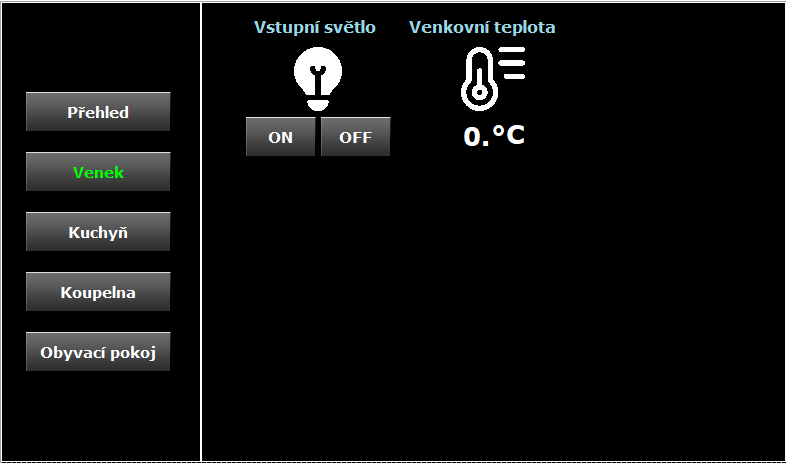
\includegraphics[scale=0.8]{obrazky/Venek.png}
  \end{center}
  \caption[WebMaker - Obrazovka venek]{WebMaker - Obrazovka venek}
  \label{fig:venek}
\end{figure}
\begin{figure}[!ht]
  \begin{center}
  \includegraphics[scale=0.8]{obrazky/koupelna.png}
  \end{center}
  \caption[WebMaker - Obrazovka koupelna]{WebMaker - Obrazovka koupelna}
  \label{fig:koupelna}
\end{figure}
\begin{figure}[!ht]
  \begin{center}
  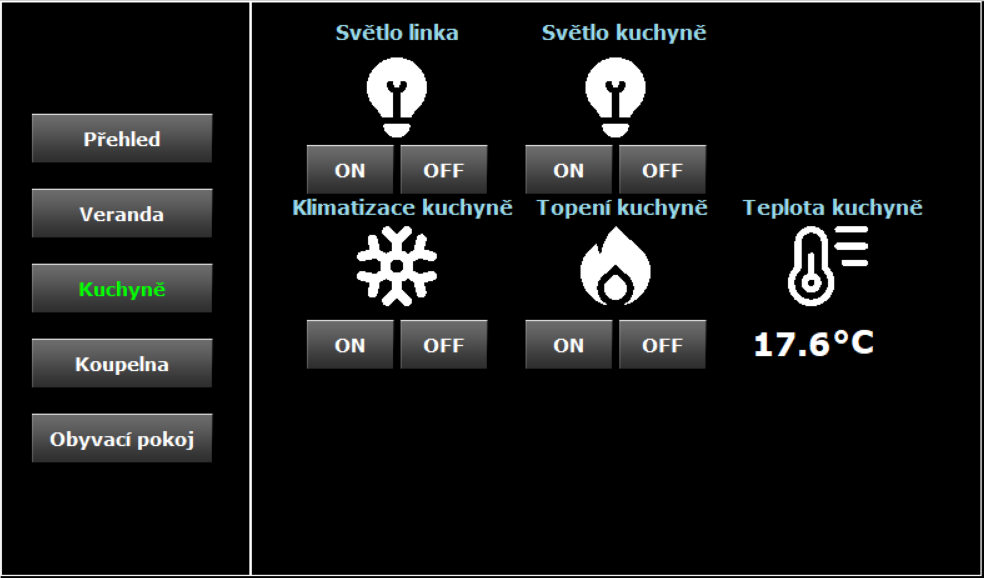
\includegraphics[scale=0.8]{obrazky/Kuchyň.png}
  \end{center}
  \caption[WebMaker - Obrazovka kuchyně]{WebMaker - Obrazovka kuchyně}
  \label{fig:kuchyn}
\end{figure}
\begin{figure}[!ht]
  \begin{center}
  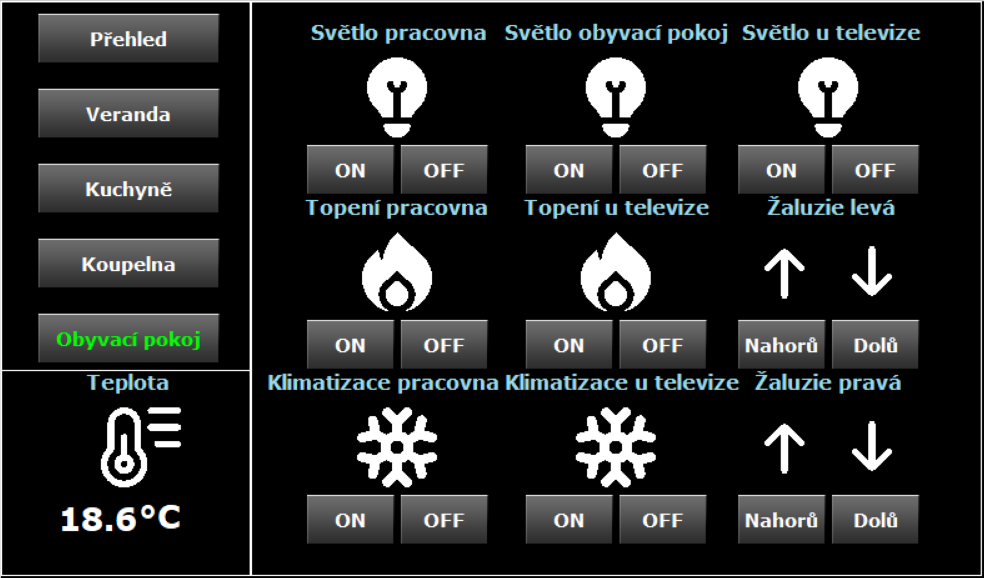
\includegraphics[scale=0.8]{obrazky/Obyvaci_pokoj.png}
  \end{center}
  \caption[WebMaker - Obrazovka obyvací pokoj]{WebMaker - Obrazovka obyvací pokoj}
  \label{fig:obyvak}
\end{figure}
\chapter{Portainer YAML}
\label{apend:portainer}
\chapter{Stack YAML}
\label{apend:stackyaml}